% Options for packages loaded elsewhere
\PassOptionsToPackage{unicode}{hyperref}
\PassOptionsToPackage{hyphens}{url}
\PassOptionsToPackage{dvipsnames,svgnames,x11names}{xcolor}
%
\documentclass[
  letterpaper,
  DIV=11,
  numbers=noendperiod]{scrartcl}

\usepackage{amsmath,amssymb}
\usepackage{iftex}
\ifPDFTeX
  \usepackage[T1]{fontenc}
  \usepackage[utf8]{inputenc}
  \usepackage{textcomp} % provide euro and other symbols
\else % if luatex or xetex
  \usepackage{unicode-math}
  \defaultfontfeatures{Scale=MatchLowercase}
  \defaultfontfeatures[\rmfamily]{Ligatures=TeX,Scale=1}
\fi
\usepackage{lmodern}
\ifPDFTeX\else  
    % xetex/luatex font selection
\fi
% Use upquote if available, for straight quotes in verbatim environments
\IfFileExists{upquote.sty}{\usepackage{upquote}}{}
\IfFileExists{microtype.sty}{% use microtype if available
  \usepackage[]{microtype}
  \UseMicrotypeSet[protrusion]{basicmath} % disable protrusion for tt fonts
}{}
\makeatletter
\@ifundefined{KOMAClassName}{% if non-KOMA class
  \IfFileExists{parskip.sty}{%
    \usepackage{parskip}
  }{% else
    \setlength{\parindent}{0pt}
    \setlength{\parskip}{6pt plus 2pt minus 1pt}}
}{% if KOMA class
  \KOMAoptions{parskip=half}}
\makeatother
\usepackage{xcolor}
\setlength{\emergencystretch}{3em} % prevent overfull lines
\setcounter{secnumdepth}{5}
% Make \paragraph and \subparagraph free-standing
\makeatletter
\ifx\paragraph\undefined\else
  \let\oldparagraph\paragraph
  \renewcommand{\paragraph}{
    \@ifstar
      \xxxParagraphStar
      \xxxParagraphNoStar
  }
  \newcommand{\xxxParagraphStar}[1]{\oldparagraph*{#1}\mbox{}}
  \newcommand{\xxxParagraphNoStar}[1]{\oldparagraph{#1}\mbox{}}
\fi
\ifx\subparagraph\undefined\else
  \let\oldsubparagraph\subparagraph
  \renewcommand{\subparagraph}{
    \@ifstar
      \xxxSubParagraphStar
      \xxxSubParagraphNoStar
  }
  \newcommand{\xxxSubParagraphStar}[1]{\oldsubparagraph*{#1}\mbox{}}
  \newcommand{\xxxSubParagraphNoStar}[1]{\oldsubparagraph{#1}\mbox{}}
\fi
\makeatother


\providecommand{\tightlist}{%
  \setlength{\itemsep}{0pt}\setlength{\parskip}{0pt}}\usepackage{longtable,booktabs,array}
\usepackage{calc} % for calculating minipage widths
% Correct order of tables after \paragraph or \subparagraph
\usepackage{etoolbox}
\makeatletter
\patchcmd\longtable{\par}{\if@noskipsec\mbox{}\fi\par}{}{}
\makeatother
% Allow footnotes in longtable head/foot
\IfFileExists{footnotehyper.sty}{\usepackage{footnotehyper}}{\usepackage{footnote}}
\makesavenoteenv{longtable}
\usepackage{graphicx}
\makeatletter
\newsavebox\pandoc@box
\newcommand*\pandocbounded[1]{% scales image to fit in text height/width
  \sbox\pandoc@box{#1}%
  \Gscale@div\@tempa{\textheight}{\dimexpr\ht\pandoc@box+\dp\pandoc@box\relax}%
  \Gscale@div\@tempb{\linewidth}{\wd\pandoc@box}%
  \ifdim\@tempb\p@<\@tempa\p@\let\@tempa\@tempb\fi% select the smaller of both
  \ifdim\@tempa\p@<\p@\scalebox{\@tempa}{\usebox\pandoc@box}%
  \else\usebox{\pandoc@box}%
  \fi%
}
% Set default figure placement to htbp
\def\fps@figure{htbp}
\makeatother
% definitions for citeproc citations
\NewDocumentCommand\citeproctext{}{}
\NewDocumentCommand\citeproc{mm}{%
  \begingroup\def\citeproctext{#2}\cite{#1}\endgroup}
\makeatletter
 % allow citations to break across lines
 \let\@cite@ofmt\@firstofone
 % avoid brackets around text for \cite:
 \def\@biblabel#1{}
 \def\@cite#1#2{{#1\if@tempswa , #2\fi}}
\makeatother
\newlength{\cslhangindent}
\setlength{\cslhangindent}{1.5em}
\newlength{\csllabelwidth}
\setlength{\csllabelwidth}{3em}
\newenvironment{CSLReferences}[2] % #1 hanging-indent, #2 entry-spacing
 {\begin{list}{}{%
  \setlength{\itemindent}{0pt}
  \setlength{\leftmargin}{0pt}
  \setlength{\parsep}{0pt}
  % turn on hanging indent if param 1 is 1
  \ifodd #1
   \setlength{\leftmargin}{\cslhangindent}
   \setlength{\itemindent}{-1\cslhangindent}
  \fi
  % set entry spacing
  \setlength{\itemsep}{#2\baselineskip}}}
 {\end{list}}
\usepackage{calc}
\newcommand{\CSLBlock}[1]{\hfill\break\parbox[t]{\linewidth}{\strut\ignorespaces#1\strut}}
\newcommand{\CSLLeftMargin}[1]{\parbox[t]{\csllabelwidth}{\strut#1\strut}}
\newcommand{\CSLRightInline}[1]{\parbox[t]{\linewidth - \csllabelwidth}{\strut#1\strut}}
\newcommand{\CSLIndent}[1]{\hspace{\cslhangindent}#1}

\usepackage{float}
\KOMAoption{captions}{tableheading}
\makeatletter
\@ifpackageloaded{caption}{}{\usepackage{caption}}
\AtBeginDocument{%
\ifdefined\contentsname
  \renewcommand*\contentsname{Table of contents}
\else
  \newcommand\contentsname{Table of contents}
\fi
\ifdefined\listfigurename
  \renewcommand*\listfigurename{List of Figures}
\else
  \newcommand\listfigurename{List of Figures}
\fi
\ifdefined\listtablename
  \renewcommand*\listtablename{List of Tables}
\else
  \newcommand\listtablename{List of Tables}
\fi
\ifdefined\figurename
  \renewcommand*\figurename{Figure}
\else
  \newcommand\figurename{Figure}
\fi
\ifdefined\tablename
  \renewcommand*\tablename{Table}
\else
  \newcommand\tablename{Table}
\fi
}
\@ifpackageloaded{float}{}{\usepackage{float}}
\floatstyle{ruled}
\@ifundefined{c@chapter}{\newfloat{codelisting}{h}{lop}}{\newfloat{codelisting}{h}{lop}[chapter]}
\floatname{codelisting}{Listing}
\newcommand*\listoflistings{\listof{codelisting}{List of Listings}}
\makeatother
\makeatletter
\makeatother
\makeatletter
\@ifpackageloaded{caption}{}{\usepackage{caption}}
\@ifpackageloaded{subcaption}{}{\usepackage{subcaption}}
\makeatother

\usepackage{bookmark}

\IfFileExists{xurl.sty}{\usepackage{xurl}}{} % add URL line breaks if available
\urlstyle{same} % disable monospaced font for URLs
\hypersetup{
  pdftitle={Detecting arrhythmia from exercise data (DRAFT)},
  pdfauthor={Ian Green \& Mark Dayer},
  colorlinks=true,
  linkcolor={blue},
  filecolor={Maroon},
  citecolor={Blue},
  urlcolor={Blue},
  pdfcreator={LaTeX via pandoc}}


\title{Detecting arrhythmia from exercise data (DRAFT)}
\author{Ian Green \& Mark Dayer}
\date{2025-06-07}

\begin{document}
\maketitle

\renewcommand*\contentsname{Table of contents}
{
\hypersetup{linkcolor=}
\setcounter{tocdepth}{3}
\tableofcontents
}

\pagebreak

\section{ABSTRACT}\label{abstract}

\subsection{Introduction}\label{introduction}

This study explores the feasibility of using heart rate data as
frequently captured by keen amateur cyclists during exercise to detect
the presence of heart rhythm problems.

\subsection{Methods}\label{methods}

Data is gathered from an existing project that is used by over 1,000
(mainly) amateur athletes to compare the cardiac stress accrued through
exercise with that of their anonymised peers. ``Gappiness'' in observed
heart rate levels is defined and its frequent presence at the top end of
the heart rate range is tested for association with athlete reports of
arrhythmia obtained through a survey.

\subsection{Results}\label{results}

In an analysis of over 130,000 activities from 189 athletes who
responded to the survey, a statistically significant association was
found between observed heart rate gappiness and reported arrhythmia,
both in a point-biserial correlation check (p-value = 0.005) and a
logistic regression (p-value = 0.01).

\subsection{Discussion}\label{discussion}

This association has a specificity of 97.6\% and a positive predictive
value of 62.5\%. For an athlete for whom this predicts arrhythmia it
would be worthwhile to seek a medical consultation. However, the
sensitivity is low so a failure to predict arrhythmia is no reassurance
that there is in fact no heart rhythm issue. This is to be expected as
we only know whether survey respondents report having or having ever had
a heart rhythm problem. Some of those who report a problem may have been
treated prior to recording the activities analysed and conversely for
others the onset may have been recent so many of their recorded
activities may pre-date the condition. We surmise that heart rate
readings recorded using chest straps are more likely to detect
arrhythmia with this method than those recorded with smart watches
measuring heart rate optically at the wrist; we note that cyclists more
frequently use the former and runners the latter.

\subsection{Conclusion}\label{conclusion}

Heart rhythm problems are increasingly observed in people who engage in
high levels of endurance sports over many years, especially cyclists. A
technique that can sometimes detect arrhythmia using data already
collected during sport is therefore of potential merit. Further
investigation, including into the evolution of changes in gappiness
before, during and after the onset of heart rhythm problems as well as
the extension to a wider pool of athletes, would appear to be
worthwhile.

\section{INTRODUCTION}\label{introduction-1}

People who regularly engage in endurance sports activities such as
cycling and running accrue from them a wide range of health benefits.
However, there is also increasing evidence that people, especially men,
who participate in high levels of such sports over many years have an
elevated likelihood of developing heart rhythm problems such as atrial
fibrillation (Christoper Case 2017); (Centurión 2019); (Calvo 2016).
This is particularly well-documented for cyclists (Baldesberger 2008).
We may surmise, although it has no bearing on our analysis, that this
could arise in part from the fact that, unlike other endurance athletes,
cyclists regularly engage in sessions of high cardiac intensity lasting
a number of hours during which the unfelt strain on the heart is not
accompanied by a felt and fatiguing strain on skeletal muscles, owing to
the mechanical advantage of being on a bike. Early diagnosis of
arrhythmias is considered important and can improve clinical outcomes
(Amara 2015); (Kirchhof 2009).

Increasingly wearable devices are being used to detect arrhythmias
(Marco V. Perez 2019); (Tison et al. 2018). It is now commonly the case
that keen endurance athletes will use a device such as a smart watch or
a bike computer with a chest strap to measure their heart rate during
exercise and record this activity on a sports website such as Strava
(www.strava.com), TrainingPeaks (www.trainingpeaks.com) or Garmin
Connect (https://connect.garmin.com). We hypothesized that it would be
possible to detect arrhythmias by an analysis of saved heart rate data.
We therefore looked for irregularities in heart rate, as detected by
smartwatches and chest straps during exertion, to see whether they
occured more frequently in athletes who self-reported heart rhythm
problems.

In observing the heart rate response of athletes wearing chest straps to
effort during exercise, we note that at the highest effort heart rates
increase towards the highest value, and in a hard session the heart rate
will generally rise \emph{smoothly} to the maximum value at around the
time of greatest effort (studying both heart rate and power data shows
that the heart rate usually lags effort by around 20 to 30 seconds). The
highest heart rate levels vary by athlete and are generally in the order
of 200 beats per minute (bpm). (The rule of thumb that \emph{maximum
heart rate = 220 - age} does not account well for the seasoned athletes
we have studied - see appendix, \emph{Analysis of strap artefacts seen
in heart rate readings} and also (Hirofumi Tanaka 2001).) However, with
unexpected frequency we also sometimes observe a jumpiness at the top
end of the heart rate chart. This can either be seen as a gap of a few
beats per minute - say from 190 bpm to 195 bpm - or as a jump to a far
higher value - say 254 bpm.

It is tempting to say that these readings, especially in the latter
category of large jumps to high values, are simply strap errors; and
they evidently sometimes are. However, we hypothesise that they can
nonetheless be informational. The chest strap is, like an ECG,
continuously sampling current in the heart muscle, which it
algorithmically converts into an instantaneous heart rate reading. The
frequency of sampling and the algorithm for translating the electrical
signal into a bpm reading are proprietary and held as secrets by
equipment manufacturers. Nonetheless, we may surmise that the pattern of
measured current from an athlete who is, for example, undergoing ectopic
beats or exhibiting anomalous electrical activity in the heart might be
expected to cause irregularity in the heart rate reported by the strap.
We therefore look for such irregularities to see whether they occur more
frequently in athletes who report heart rhythm problems. If they do and
if we are able to establish a meaningful association, we may be able to
alert athletes to seek a medical consultation as soon as such a pattern
becomes evident.

\section{METHODS}\label{methods-1}

\subsection{Data acquisition}\label{data-acquisition}

The data that is used in this study is from the Crickles project, whose
purpose is to collect data from amateur endurance athletes and analyse
the extent of ``cardiac stress'' accrued through activities such as
cycling and running. Data from athletes who sign up to Crickles is
collected from the popular website Strava.com. Athletes who wish to
participate in the Crickles project enroll by hitting the \emph{Connect
with Strava} button on the website http://crickles.org. This authorises
the Crickles software to access the athlete's data. Crickles then does
an initial load of some years of historical data and adds the athlete to
the ongoing update.

Crickles performs a range of analyses on this data, the results of which
are securely stored on Crickles AWS Cloud servers. Each athlete can
access analysis on their own activities in comparision with the
anonymised data of all other Crickles participants through the
\emph{Crickles Navigator} website http://navigator.crickles.org.

Throughout this paper the term ``activity'' is used in the natural sense
of a single, complete sport session recorded by an athlete who defines
its duration by starting their sports device at the start of the session
and stopping it at the end.

Crickles is purely a research platform. It does not charge users, nor
does it raise money by selling on users' data or in any other way.
Athletes can unauthorise Crickles' access to their data at any time.
Recently, Crickles users were asked to voluntarily complete a survey to
facilitate the research into the detection of arrhythmias.

\subsection{Heart health Survey
Questionnaire}\label{heart-health-survey-questionnaire}

Crickles users were invited to complete a short questionnaire that
captured information about their cardiac health. Questions include
whether they have arrhythmia or diabetes, been prescribed beta blockers,
experienced chest pain, fainted or had a heart attack. To date, 236
athletes have completed the survey. A few of these either don't have any
activities loaded by Crickles or only have activities without heart rate
data; excluding those gives us 228 athletes whose heart rate data we can
analyse in conjunction with their heart health data.

The only response that we use from the survey is to the question,
\emph{Do you have, or have you had a heart rhythm problem?}.

\subsection{Analysis of the Heart Rate
Data}\label{analysis-of-the-heart-rate-data}

We aimed to determine if persistent observable irregularities in the
heart rate data might be more prevalent in those with a self reported
history of arrhythmia. To this end we want to clean the data of readings
that are wrong in uninteresting ways while discarding as little as
possible that may prove useful.

We begin with two measures of the regularity of the heart rate chart for
any given activity. The first is \textbf{stickiness}. We observe (see
Appendix) that sometimes the heart rate reading jams on a certain value
for an implausibly long period of time. Where this happens, we believe
it to be an error on the part of the recording sports device. Moreover,
it is unlikely to be an \emph{interesting} error in which the athlete's
cardiac behaviour plays any part. From the perspective of experience, we
might expect that any record of a heart rate held at the same level for
over a minute is wrong: while the fluctuation of, say, someone cycling
at threshold in a time trial might be low, we would expect to see some
change over the course of any minute. If we look at the actual record of
reported sustained heart rates, there is a wide range of values; the
maximum currently stands at over 37 hours! However, 95\% of the range is
within 90 seconds and so we take this as our threshold for reporting a
probable error. Here is the distribution of values that are less than 90
seconds:

\begin{verbatim}
Warning: The dot-dot notation (`..count..`) was deprecated in ggplot2 3.4.0.
i Please use `after_stat(count)` instead.
\end{verbatim}

\begin{figure}[H]

{\centering \pandocbounded{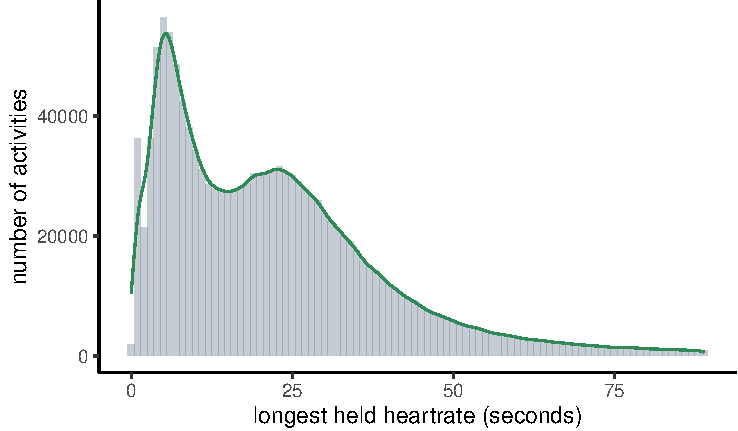
\includegraphics[keepaspectratio]{arrhythmia_files/figure-pdf/sticky-1.pdf}}

}

\caption{Stickiness frequency}

\end{figure}%

We call an activity in which we see a stuck heart rate value for longer
than 90 seconds \textbf{sticky}. On the Crickles Navigator these
activities are flagged \textbf{Check\_Strap}.

For our second measure, we're interested in how jumpy the heart rate
chart is. This is potentially much more interesting physiologically as
an erratic heart rate may well be indicative of some kind of a
pathology. The study of time series volatility is an advanced science
and there are many techniques that we could deploy for measurement. For
example, we might use a stochastic volatility model with a jump process
to fit the patterns that we see (Zou 2014). However, the nature of
athletic exercise and the limitations of the sports devices mitigate
against several of these. To take some examples:

\begin{enumerate}
\def\labelenumi{\arabic{enumi}.}
\tightlist
\item
  Keen athletes quite often engage in High Intensity Interval Training
  (HIIT) sessions. A typical protocol might be to ride at maximum effort
  on a turbo trainer for 30 seconds then rest for 30 seconds then
  repeat, and to do this in blocks of ten repetitions with a recovery
  break between each block.
\item
  Different sports devices record the heart rate at different sampling
  frequencies. Typically, a sports watch will sample infrequently at low
  heart rates and more frequently at high heart rates to prolong battery
  life. In contrast, a bike computer that records power from a power
  meter as well as heart rates will usually sample every second. The
  method that the device chooses for sampling the data is set by a
  combination of undocumented logic intrinsic to each device and,
  sometimes, configuration variables that can be set by the device
  owner. We do not have knowledge of either what sports device is being
  used or of how it is configured.
\item
  All sports devices are prone to \emph{contact failures} with the skin.
  It's therefore reasonably common to see wrong readings towards the
  start of a bike ride when a cyclist is speeding downhill; at this time
  with little effort and no sweat build-up and the compounding effect of
  a jersey flapping against a chest strap, wrong high readings are
  sometimes seen.
\item
  As we saw above, sports devices reasonably often show high readings
  that are simply higher than we believe can be correct.
\end{enumerate}

Points 1 and 2 present technical challenges to certain volatility
models. Points 3 and 4 challenge any volatility model by the
introduction of plainly wrong data; however, these phenomena, especially
point 4, may potentially be responsive to electrical activity in the
heart and even where the readings are numerically wrong they may carry
signal value: the fact that the sports device is reporting a wrong value
may itself be diagnostic! Unlike sticky readings, we therefore will not
wish to discard them.

Both the variable and unknown sampling regimes of devices and especially
the entanglement of potentially signal-bearing errors with the true
heart rate data render the use of time series volatility models
problematic. Instead, we might turn to pattern matching algorithms. In
principle, we could split each heart rate chart into a set of short
heart rate sequences, parametrise these in some way and then use a
machine learning technique to hunt for assocations with arrhythmia.
While this is likely to be complex, computationally expensive and
opaque, it remains open to us as a future research direction when we
have a larger data set of survey responses.

Here, we rely on a simpler approach. We formulate a flag for determining
whether or not a heart rate chart in its entirety is erratic by
introducing the concept of the \emph{natural maximum} heart rate for an
activity. This is calculated by looking for gaps in the range of
observed heart rate readings over the modal value. The reasoning behind
this is that at higher heart rate levels the athlete's heart rate
typically steps up and down one bpm at a time, and certainly we don't
normally observe discountinuities in the range of heart rates attained.

If there are no such gaps the natural maximum for the activity is equal
to the actual observed maximum. If there are such gaps then the natural
maximum is the heart rate level immediately below the lowest such gap.
We hypothesise that the gaps most likely to be indicative of arrhythmia
are those that occur when the athlete is under exertion. In the course
of other analysis not covered in this paper we make a running estimate
of the Lactate Threshold Heart Rate (LTHR) of each athlete. (As an
alternative, LTHR can be roughly approximated as a percentage of the
athlete's maximum heart rate.) We call an activity for which the maximum
heart rate exceeds the natural maximum and during which the athlete's
heart rate also exceeds his or her prevailing LTHR \textbf{gappy}; the
quality of being gappy is \textbf{gappiness}.

Here's an example of a typical gappy heart rate chart:

\begin{figure}[H]

{\centering \pandocbounded{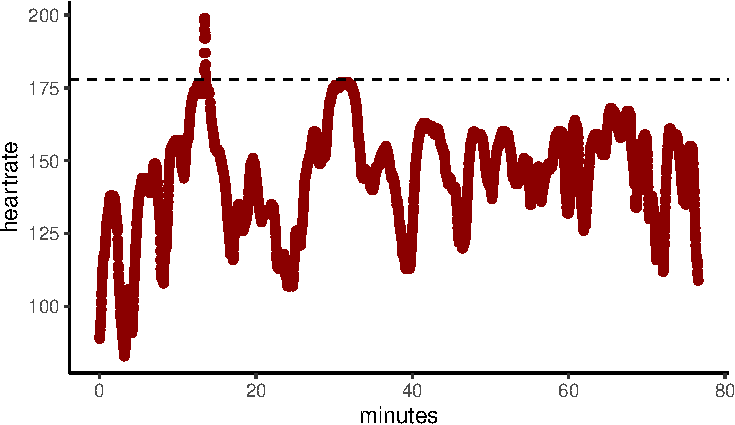
\includegraphics[keepaspectratio]{arrhythmia_files/figure-pdf/gappy_chart-1.pdf}}

}

\caption{An example of gappiness}

\end{figure}%

Clearly, something unusual is happening for the burst in which the heart
rate pops above the line, drawn at 178bpm. If we zoom in on the four
minute period around the burst we see this:

\begin{figure}[H]

{\centering \pandocbounded{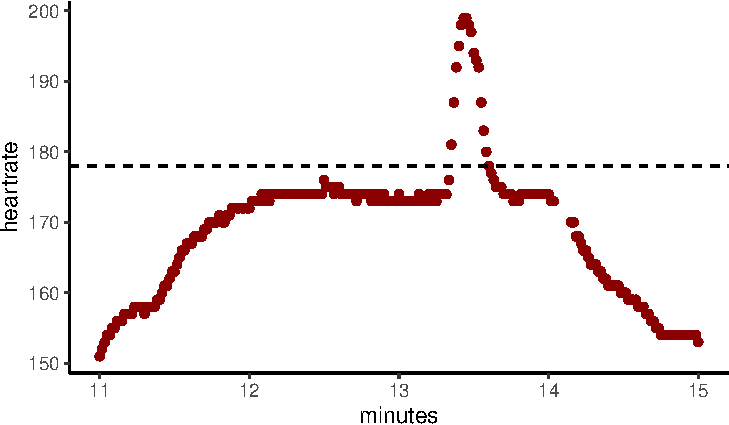
\includegraphics[keepaspectratio]{arrhythmia_files/figure-pdf/gappy_chart_zoom-1.pdf}}

}

\caption{Gappiness at per second resolution}

\end{figure}%

Here, 178bpm is the \emph{natural maximum}. We can't know whether the
little spike is a faithful reading of the athlete's heart rate or a blip
in the device, and, if the latter, whether or not the blip was caused by
electrical cardiac activity. On its own, this incident has no medical
significance. However, we have hundreds or thousands of such records for
most athletes and we hypothesise that when such spikes occur with
heightened frequency for an athlete it may be associated with
arrhythmia.

Here are a couple more examples from a different athlete:

\begin{figure}[H]

{\centering \pandocbounded{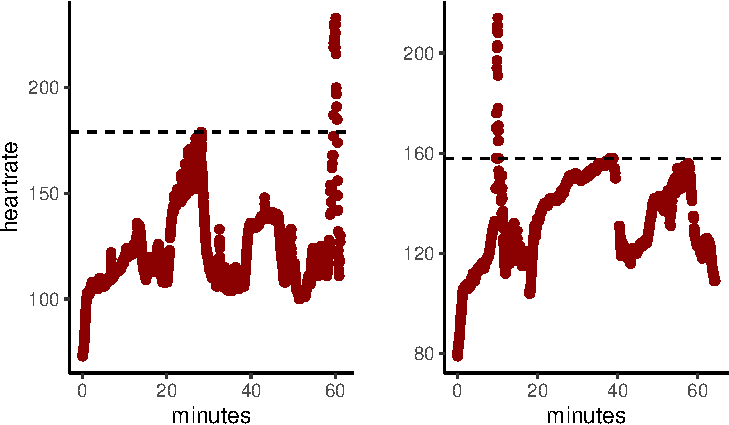
\includegraphics[keepaspectratio]{arrhythmia_files/figure-pdf/gappy_chart_2more-1.pdf}}

}

\caption{Further examples of gappiness}

\end{figure}%

As a further filter to remove activities where we have reason to believe
that gappiness is occuring due to a limitation or fault in the device,
we consider also the low end of the heart rate range. By analogy with
the natural maximum, we can also find the \emph{natural minimum} heart
rate for an activity: this is the level above which the observed heart
rate range is complete up to the modal value. It is reasonably common to
see a running activity recorded with a sports watch show a natural
minimum heart rate above the actual minimum as the watch takes some
seconds to catch up with the initial exertion of the athlete.

Finally, here's an example where gappiness breaks out in a sequence of
efforts during an interval session:

\begin{figure}[H]

{\centering \pandocbounded{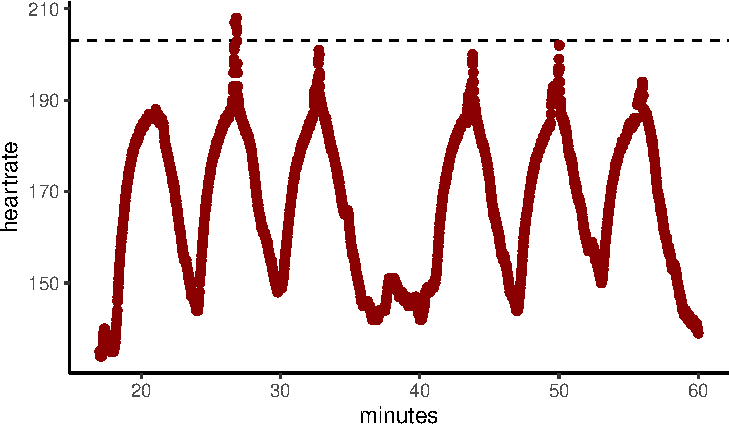
\includegraphics[keepaspectratio]{arrhythmia_files/figure-pdf/gappy_repeated-1.pdf}}

}

\caption{Repeated gappiness during intervals}

\end{figure}%

While gaps at the low end are logically independent and of a different
character from gaps at the high end, as a precaution when an activity
that is gappy at the high end is also gappy at the low end we flag it
differently. Here's an example of an activity that is gappy at both
ends:

\begin{figure}[H]

{\centering \pandocbounded{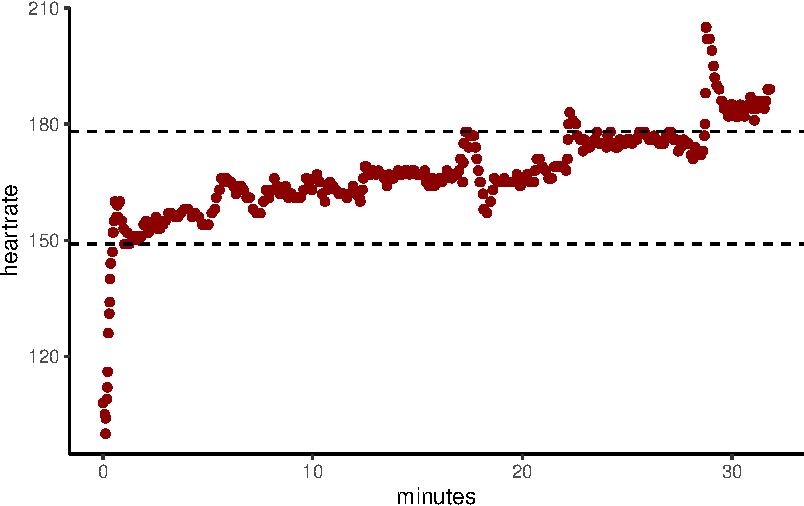
\includegraphics[keepaspectratio]{arrhythmia_files/figure-pdf/unclear-1.pdf}}

}

\caption{Example of an unclear activity}

\end{figure}%

Activities that are not sticky and that are gappy at the high end but
not at the low end are flagged as \textbf{irregular}. Gappy non-sticky
activities that are gappy at both the high and the low ends are marked
as \textbf{unclear}.

Activities that are neither sticky (flagged as \emph{Check\_Strap}),
irregular or unclear are marked as \textbf{regular}. Whereas a
volatility metric or a machine learning algorithm could give us a
\emph{degree} of irregularity for an activity, this methodology simply
tells us \emph{whether or not} an activity appears irregular. We rely on
the frequency of such readings to give us a continuous measure for an
athlete.

This table gives an indication of the frequency of incidence of these
phenomena:

\begin{longtable}[]{@{}lrr@{}}
\caption{Regularity - counts and percentages}\tabularnewline
\toprule\noalign{}
Category & count & percentage \\
\midrule\noalign{}
\endfirsthead
\toprule\noalign{}
Category & count & percentage \\
\midrule\noalign{}
\endhead
\bottomrule\noalign{}
\endlastfoot
Regular & 1,204,160 & 86.4 \\
Unclear & 91,817 & 6.6 \\
Check\_Strap & 72,984 & 5.2 \\
Irregular & 25,267 & 1.8 \\
\end{longtable}

The category of any particular activity carries low informational value.
However, we believe that when aggregated by athlete there is scope for
significance to arise. On a prosaic level, when the proportion of an
athlete's activities that report Check\_Strap rises well above the
population average we can propose that it may be time to consider
getting a new strap (or relevant sports device).

The more interesting questions arise from an exploration of supra-normal
frequencies of activities flagged as irregular.

First we make a detour to consider the sport(s) that will be the focus
for the remainder of this analysis.

\subsection{Focus on cycling and chest
straps}\label{focus-on-cycling-and-chest-straps}

We would like to restrict our study to cyclists using chest straps.
Selecting only cyclists is straightforward; we can also include cyclists
using turbo trainers and those on platforms such as Zwift that offer
``virtual rides''. Selecting only activities in which a chest strap was
used is more problematic. This is because it is possible for an athlete
to use one device to collect and record the data and another to measure
the heart rate. For example, when using a Garmin Forerunner sports watch
the heart rate can be measured either from the in-built optical heart
rate monitor or from a chest strap. Likewise, while most cyclists using
a bike computer will measure their heart rate (if they do so at all)
using a chest strap, it is nonetheless possible for them to use a sports
watch for the purpose and to connect the two using bluetooth. From the
data available to us, even though we can sometimes find the name of one
``device'' that was used on an activity, we have no failsafe way of
knowing which device was used to record the heart rate. For example, in
an extreme case in which a cyclist on a Taxc Neo turbo trainer records a
ride on the software platform Zwift using a Wahoo Elemnt bike computer
and measures his or her heart rate with a Garmin Forerunner watch, four
``devices'' are being used and we know, at best, the name of only one of
them, and it probably won't be the Forerunner.

There are, though, \emph{de facto} correlations between exercise types
and equipment. Looking only at runs, rides and virtual rides and
classifying each device into a ``device family'', we analysed the
frequency of use on a random sample of over 10,000 activities:

\begin{longtable}[]{@{}lrrr@{}}
\caption{Sample count by device family and sport}\tabularnewline
\toprule\noalign{}
device\_family & Ride & Run & VirtualRide \\
\midrule\noalign{}
\endfirsthead
\toprule\noalign{}
device\_family & Ride & Run & VirtualRide \\
\midrule\noalign{}
\endhead
\bottomrule\noalign{}
\endlastfoot
bike\_computer & 5,945 & 6 & 15 \\
phone & 214 & 9 & 0 \\
platform & 121 & 0 & 1,446 \\
trainer & 116 & 0 & 16 \\
watch & 770 & 897 & 10 \\
\end{longtable}

We see that in this sample, the large majority of cyclists on
non-virtual rides used bike computers, almost all runners used sports
watches and most virtual rides took place on platforms such as Zwift or
Trainer Road. Even though we don't know how many of the runners also
used chest straps as well as sports watches or how many of the cyclists
took heart rate readings from a watch, we believe that the use of chest
straps is more prevalent than watches for heart rate recording amongst
cyclists as it would be duplicative, inconvenient and of little obvious
benefit to use both a bike computer and a sports watch at the same time.
Furthermore, as keen cyclists ourselves, this is what the authors
consistently observe.

More information on the use of various types of device is supplied in
the appendix, \emph{Analysis of device by sport}.

\subsection{Unreliable straps}\label{unreliable-straps}

The table above showed us the overall proportion of activities that are
flagged with Check\_Strap. When we break this down to find the ratio for
each athlete and plot the distribution of ratios we get this:

\begin{figure}[H]

{\centering \pandocbounded{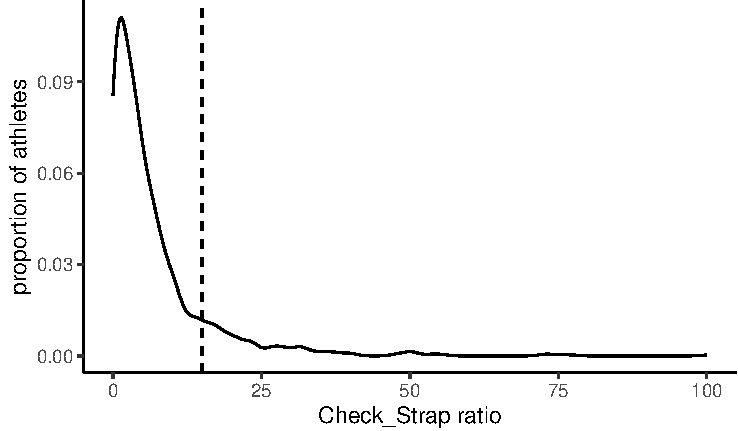
\includegraphics[keepaspectratio]{arrhythmia_files/figure-pdf/strap_athlete-1.pdf}}

}

\caption{Frequency of `Check Strap'}

\end{figure}%

There is a non-normal distribution of values with a median of 3.94\% and
a mean of 6.85\%. The distribution falls monotonically from the mode
until about 15\%, which we have marked with a dotted line. We hypthosise
that the athletes represented by ratios to the right of the line are
likely to be repeatedly exercising with sports devices (possibly chest
straps) that are consistently not working. We therefore removed these
athletes from our sample.

Paring down to only cycling activities for which we have heart rate data
and removing the higher-error athletes still leaves us with 1085
athletes and 813,633 activities. Next, we have to restrict our focus
much further.

\section{RESULTS}\label{results-1}

\subsection{Irregularity and
arrhythmia}\label{irregularity-and-arrhythmia}

Is frequency of \textbf{irregular} activities associated with a
diagnosis of arrhythmia in cyclists? To answer that question we need to:

\begin{enumerate}
\def\labelenumi{\arabic{enumi}.}
\tightlist
\item
  calculate the ratio of activities marked as \textbf{irregular} for
  each cyclist in our reduced population;
\item
  find those for whom we have a survey response - this is a large
  reduction in data;
\item
  test the association strength between each athlete's \emph{irregular
  ratio} and the presence/absence of an arrhythmia diagnosis.
\end{enumerate}

Steps 1 and 2 are simply data manipulation. Since we don't believe
sticky activities to be informational and we're uncertain about unclear
ones, we set our \emph{irregular ratio} to be the proportion of
activities marked \emph{irregular} of those marked either
\emph{irregular} or \emph{regular}.

At this point we have reduced our survey population down to 212
athletes. Of these, 60 (28.3\%) report having an arrhythmia diagnosis.
This is a high percentage, which we can attribute to a strong selection
bias amongst those who choose to complete the survey.

The distribution of irregular ratios is shown by a Shapiro test to be
significantly non-normal, which is not surprising.

We can compare the irregular ratios for athletes with and without
arrhythmia:

\begin{figure}[H]

{\centering \pandocbounded{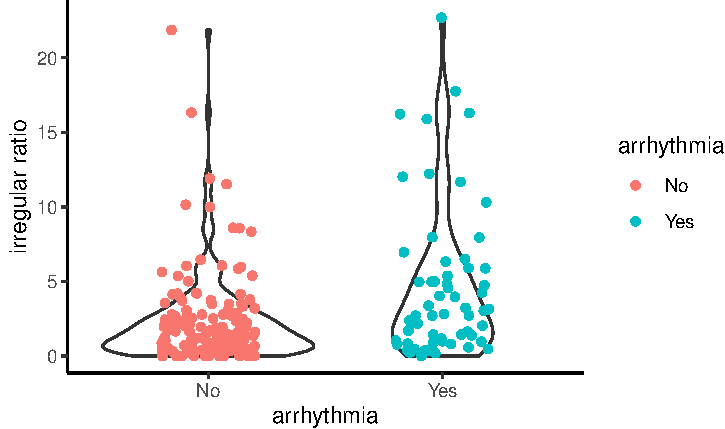
\includegraphics[keepaspectratio]{arrhythmia_files/figure-pdf/irreg_chart-1.pdf}}

}

\caption{A violin plot comparing irregular ratios for athletes with and
without arrhythmia}

\end{figure}%

The non-arrhythmics tend to clump on the low ratios whereas the
arrhythmics have a higher proportion of elevated values.

As a first check of whether this is supported statistically, we can run
a point-biserial correlation check; here \emph{arr\_num} is 1 for
athletes who have a diagnosis of arrhythmia and 0 for those who don't:

\begin{verbatim}

    Pearson's product-moment correlation

data:  survey_results$irreg_ratio and survey_results$arr_num
t = 4.0299, df = 210, p-value = 7.801e-05
alternative hypothesis: true correlation is not equal to 0
95 percent confidence interval:
 0.1381621 0.3886412
sample estimates:
      cor 
0.2679231 
\end{verbatim}

The p-value of \textbf{0} suggests that the correlation of
\textbf{26.8\%} represents a meaningful association whose probability of
being due to chance is low.

We can explore this further with a logistic regression:

\begin{longtable}[]{@{}
  >{\centering\arraybackslash}p{(\linewidth - 8\tabcolsep) * \real{0.2500}}
  >{\centering\arraybackslash}p{(\linewidth - 8\tabcolsep) * \real{0.1528}}
  >{\centering\arraybackslash}p{(\linewidth - 8\tabcolsep) * \real{0.1806}}
  >{\centering\arraybackslash}p{(\linewidth - 8\tabcolsep) * \real{0.1389}}
  >{\centering\arraybackslash}p{(\linewidth - 8\tabcolsep) * \real{0.1667}}@{}}
\caption{Fitting generalized (binomial/logit) linear model: Arrhythmia
\textasciitilde{} irreg\_ratio}\tabularnewline
\toprule\noalign{}
\begin{minipage}[b]{\linewidth}\centering
~
\end{minipage} & \begin{minipage}[b]{\linewidth}\centering
Estimate
\end{minipage} & \begin{minipage}[b]{\linewidth}\centering
Std. Error
\end{minipage} & \begin{minipage}[b]{\linewidth}\centering
z value
\end{minipage} & \begin{minipage}[b]{\linewidth}\centering
Pr(\textgreater\textbar z\textbar)
\end{minipage} \\
\midrule\noalign{}
\endfirsthead
\toprule\noalign{}
\begin{minipage}[b]{\linewidth}\centering
~
\end{minipage} & \begin{minipage}[b]{\linewidth}\centering
Estimate
\end{minipage} & \begin{minipage}[b]{\linewidth}\centering
Std. Error
\end{minipage} & \begin{minipage}[b]{\linewidth}\centering
z value
\end{minipage} & \begin{minipage}[b]{\linewidth}\centering
Pr(\textgreater\textbar z\textbar)
\end{minipage} \\
\midrule\noalign{}
\endhead
\bottomrule\noalign{}
\endlastfoot
\textbf{(Intercept)} & -1.409 & 0.2107 & -6.688 & 2.267e-11 \\
\textbf{irreg\_ratio} & 0.146 & 0.04202 & 3.475 & 0.0005105 \\
\end{longtable}

Again, the low p-value of \textbf{0.001} for irreg\_ratio indicates a
significant relationship.

Re-running the violin plot using the fitted values from the logistic
regression model rather than the observed irregular ratios preserves the
pattern of the chart above:

\begin{figure}[H]

{\centering \pandocbounded{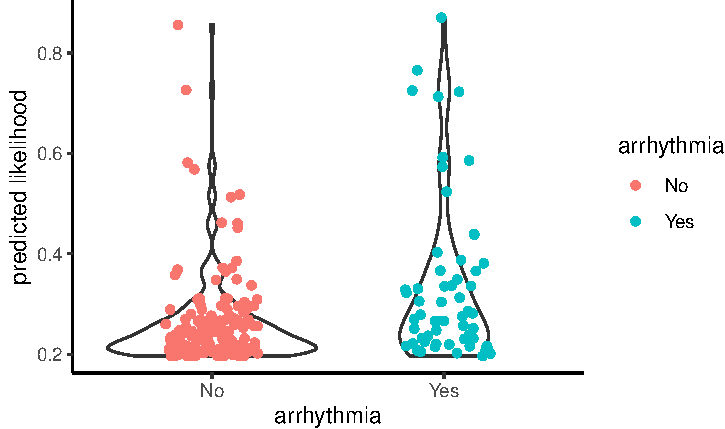
\includegraphics[keepaspectratio]{arrhythmia_files/figure-pdf/prediction_chart-1.pdf}}

}

\caption{Modelled likelihood of arrhythmia by athlete's own report}

\end{figure}%

Now we can apply the model to all of the athletes for whom we have heart
rate data from cycling but no survey response:

\begin{longtable}[]{@{}lr@{}}
\caption{Arrhythmia prediction for athletes with no survey
response}\tabularnewline
\toprule\noalign{}
predicted\_arrhythmia & n \\
\midrule\noalign{}
\endfirsthead
\toprule\noalign{}
predicted\_arrhythmia & n \\
\midrule\noalign{}
\endhead
\bottomrule\noalign{}
\endlastfoot
FALSE & 849 \\
TRUE & 23 \\
\end{longtable}

This predicts that 2.6\% of our population would have arrhythmia as
gauged by the irregular ratio.

\subsection{Confusion matrix and the utility of the
prediction}\label{confusion-matrix-and-the-utility-of-the-prediction}

The quality of fit of the logistic regression can be assessed in
headline terms by comparing the fitted probabilities of arrhythmia with
the actual values:

\begin{longtable}[]{@{}lrr@{}}
\caption{Confusion matrix for logistic regression}\tabularnewline
\toprule\noalign{}
Arrhythmia & Predict No & Predict Yes \\
\midrule\noalign{}
\endfirsthead
\toprule\noalign{}
Arrhythmia & Predict No & Predict Yes \\
\midrule\noalign{}
\endhead
\bottomrule\noalign{}
\endlastfoot
No & 146 & 6 \\
Yes & 51 & 9 \\
\end{longtable}

Sensitivity: \textbf{15\%}\\
Specificity: \textbf{96.1\%}\\
Positive Predictive Value: \textbf{60\%}\\
Negative Predictive Value: \textbf{74.1\%}

Here, \emph{Predict No} simply means the modelled probability is
\textless= 0.5 and \emph{Predict Yes} means it's over 0.5.

\subsection{Irregularity, Unclarity and
Stickiness}\label{irregularity-unclarity-and-stickiness}

We have made a number of important assumptions regarding our gappiness
and stickiness measures, notably that stickiness is unlikely to be of
physiological interest whereas gappiness is our central measure of
suspicion. We therefore would hope to find that there is no meaningful
correlation between the two.

If we run a correlation test on the irregular\_ratio and the
strap\_ratio we get the following:

\begin{longtable}[]{@{}
  >{\centering\arraybackslash}p{(\linewidth - 8\tabcolsep) * \real{0.2361}}
  >{\centering\arraybackslash}p{(\linewidth - 8\tabcolsep) * \real{0.0833}}
  >{\centering\arraybackslash}p{(\linewidth - 8\tabcolsep) * \real{0.1389}}
  >{\centering\arraybackslash}p{(\linewidth - 8\tabcolsep) * \real{0.3472}}
  >{\centering\arraybackslash}p{(\linewidth - 8\tabcolsep) * \real{0.1250}}@{}}
\caption{Pearson's product-moment correlation:
\texttt{results\$irreg\_ratio} and
\texttt{results\$strap\_ratio}}\tabularnewline
\toprule\noalign{}
\begin{minipage}[b]{\linewidth}\centering
Test statistic
\end{minipage} & \begin{minipage}[b]{\linewidth}\centering
df
\end{minipage} & \begin{minipage}[b]{\linewidth}\centering
P value
\end{minipage} & \begin{minipage}[b]{\linewidth}\centering
Alternative hypothesis
\end{minipage} & \begin{minipage}[b]{\linewidth}\centering
cor
\end{minipage} \\
\midrule\noalign{}
\endfirsthead
\toprule\noalign{}
\begin{minipage}[b]{\linewidth}\centering
Test statistic
\end{minipage} & \begin{minipage}[b]{\linewidth}\centering
df
\end{minipage} & \begin{minipage}[b]{\linewidth}\centering
P value
\end{minipage} & \begin{minipage}[b]{\linewidth}\centering
Alternative hypothesis
\end{minipage} & \begin{minipage}[b]{\linewidth}\centering
cor
\end{minipage} \\
\midrule\noalign{}
\endhead
\bottomrule\noalign{}
\endlastfoot
1.496 & 210 & 0.1362 & two.sided & 0.1027 \\
\end{longtable}

The correlation is weak at 10.3\% and the p-value of 0.136 indicates
that we cannot reject the null hypothesis (no correlation).

In contrast, and as we would expect, the irregularity ratio is highly
correlated with the ratio of Unclears:

\begin{longtable}[]{@{}
  >{\centering\arraybackslash}p{(\linewidth - 8\tabcolsep) * \real{0.2267}}
  >{\centering\arraybackslash}p{(\linewidth - 8\tabcolsep) * \real{0.0800}}
  >{\centering\arraybackslash}p{(\linewidth - 8\tabcolsep) * \real{0.2400}}
  >{\centering\arraybackslash}p{(\linewidth - 8\tabcolsep) * \real{0.3333}}
  >{\centering\arraybackslash}p{(\linewidth - 8\tabcolsep) * \real{0.1200}}@{}}
\caption{Pearson's product-moment correlation:
\texttt{results\$irreg\_ratio} and
\texttt{results\$unclear\_ratio}}\tabularnewline
\toprule\noalign{}
\begin{minipage}[b]{\linewidth}\centering
Test statistic
\end{minipage} & \begin{minipage}[b]{\linewidth}\centering
df
\end{minipage} & \begin{minipage}[b]{\linewidth}\centering
P value
\end{minipage} & \begin{minipage}[b]{\linewidth}\centering
Alternative hypothesis
\end{minipage} & \begin{minipage}[b]{\linewidth}\centering
cor
\end{minipage} \\
\midrule\noalign{}
\endfirsthead
\toprule\noalign{}
\begin{minipage}[b]{\linewidth}\centering
Test statistic
\end{minipage} & \begin{minipage}[b]{\linewidth}\centering
df
\end{minipage} & \begin{minipage}[b]{\linewidth}\centering
P value
\end{minipage} & \begin{minipage}[b]{\linewidth}\centering
Alternative hypothesis
\end{minipage} & \begin{minipage}[b]{\linewidth}\centering
cor
\end{minipage} \\
\midrule\noalign{}
\endhead
\bottomrule\noalign{}
\endlastfoot
25.54 & 210 & 2.417e-66 * * * & two.sided & 0.8698 \\
\end{longtable}

This suggests that we may, perhaps, be over-cautious in removing unclear
activities from our analysis (including them does not change the results
materially.)

\section{DISCUSSION}\label{discussion-1}

In summary we have demonstrated that using simple algorithms it may be
possible to screen cyclists for the presence or absence of an
arrhythmia. However, it was far from perfect with current technology.
Improvements in the ability of devices to record heart rate and ECGs, as
well as a bigger database of activities and subjects with and without
arrhythmia is likely to mean that algorithms developed in the future can
be expected to improve the ability to detect problems early, leading to
earlier treatment.

There are many limitations to our data. Firstly, we were unaware of the
type of arrhythmia that our subjects suffered from, and whether it was
an ongoing problem or a frequent problem, and whether/how episodes of
arrhythmia coincided with the timeframe over which we have the subject's
exercise data. Atrial fibrillation, probably the most common ``serious''
rhythm problem that afflicts cyclists and other endurance athletes, can
be a problem that surfaces rarely or be something that is consistent. A
change in medication or a procedure can also change its frequency or
severity. It is also possible that people who have a heart rhythm
problem avoid exercise on days when it is occurring or avoid particular
forms of exercise. Furthermore, some rhythm problems cause only very
fleeting interruptions in the ECG trace and would not be detected by our
methodology (for example ventricular ectopics). Some rhythm problems
become less frequent with exercise. These are reasons, perhaps, for the
relatively poor sensitivity.

\subsection{Simplicity}\label{simplicity}

A strength and a weakness of the algorithm for generating the irregular
ratio is its simplicity. Given that we have hundreds of thousands of
activity records from hundreds of athletes and typically thousands or
tens of thousands of heart rate observations for each activity, it might
be expected that a machine learning algorithm would perform better. Over
time, this may be so but for so long as we only have a relatively small
number of survey responses and the issue of identifying errors when
sports devices have mis-parsed a heart rate signal remains entangled
with the difficulty of true pattern detection, a simple algorithm that
offers good heuristics is advantageous. It also helps that it is fast
and easy to calculate.

\subsection{Limitations}\label{limitations}

As well as shortcomings in the mathematical model, there are intrinsic
limitations in the data. Notably, there are likely to be athletes who
have responded to our survey and who correctly report that they have not
being diagnosed with arrhythmia but who nonetheless have it.

We made a number of assumptions regarding our gappiness and stickiness,
notably that stickiness is unlikely to be of physiological interest
whereas gappiness is our central measure of suspicion. We confirmed,
however, that there was no correlation between the two.

If we had further details about subjects' arrhythmias, it also would
enable us to study the temporal pattern of the irregularity ratio,
which, in the context of a date of onset or diagnosis, might be expected
to be fruitful. For example, in the table given in the Confusion matrix
section above we observed a relatively large number of cases where a
survey response disclosed arrhythmia that was not predicted by the
model. At least some of these may be due to remedial measures such as
medication and/or reduction of exercise intensity consequent to
diagnosis but pre-dating the collection of many or all activities.

\section{CONCLUSION}\label{conclusion-1}

In this study we have found that in a population of around 100 very
active cyclists, a high frequency with which gaps appear at the top end
of the heart rate range is associated with heart rhythm problems. In
some instances the heart rates reported are higher than is medically
plausible. We surmise that, even when lacking fidelity to the true heart
rate, readings from a chest strap may be informational in signalling
erratic electrial cardiac activity. Where this is observed, it may prove
a useful alert to the subject to seek a medical consultation to check
for arrhythmia. On the other hand, the absence of such a pattern does
not, on the basis of the present analysis, reassure the subject that
there is no arrhythmia.

This merits further investigation, for example to: analyse changes in
irregularity ratio over time for athletes with a known medical history;
compare more sports; compare types of heart rate monitor, including
those that read a pulse optically at the wrist; apply alternative
irregularity detection techniques, including techniques that result in a
continuous regularity metric; extend to a wider pool of athletes.

\section{APPENDICES}\label{appendices}

\subsection{Data available}\label{data-available}

At the time of writing, 1291 athletes have at some point authorised
Crickles to access their data and of these 1074 currently remain
authorised and are thus available for this study. The gender breakdown
of the authorised athletes is as follows:

\begin{longtable}[]{@{}lr@{}}
\caption{Athletes by gender}\tabularnewline
\toprule\noalign{}
Gender & Count \\
\midrule\noalign{}
\endfirsthead
\toprule\noalign{}
Gender & Count \\
\midrule\noalign{}
\endhead
\bottomrule\noalign{}
\endlastfoot
F & 74 \\
M & 991 \\
NA & 9 \\
\end{longtable}

The youngest athlete is 19 years old, the eldest is 1951 years old and
the median age is 53.22.

From these athletes, we have analysed 1,876,121 activities, which arise
from 39 different sports. The activity counts for the ten most heavily
represented sports are as follows:

\begin{longtable}[]{@{}lr@{}}
\caption{Activity county of top ten sports}\tabularnewline
\toprule\noalign{}
Sport & Records \\
\midrule\noalign{}
\endfirsthead
\toprule\noalign{}
Sport & Records \\
\midrule\noalign{}
\endhead
\bottomrule\noalign{}
\endlastfoot
Ride & 960,615 \\
Run & 321,323 \\
VirtualRide & 229,419 \\
Walk & 146,953 \\
Workout & 54,188 \\
WeightTraining & 35,353 \\
Swim & 33,815 \\
Yoga & 28,865 \\
Hike & 25,235 \\
Rowing & 9,892 \\
\end{longtable}

Many, but not all, of these activities are saved with heart rate
readings recorded by the sports device throughout the activity. In fact,
the proportion of activities that have heart rate data currently stands
at 76.73\%. When estimating cardiac stress, in the absence of heart rate
data we can use statistical models based on factors such as speed, power
and gradient as a proxy; however, for the purposes of this paper we only
use those activities for which we have heart rate data.

\subsection{Analysis of strap artefacts seen in heart rate
readings}\label{analysis-of-strap-artefacts-seen-in-heart-rate-readings}

First, we look at the maximum heart rate levels recorded for each
athlete. Taking out one outlier in which a heart rate of 365 beats per
minute (bpm) was recorded, we find this distribution of maximum heart
rates by athlete:

\begin{figure}[H]

{\centering \pandocbounded{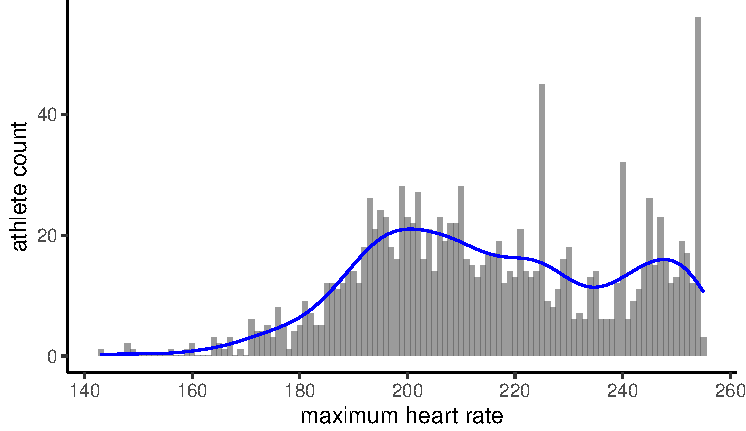
\includegraphics[keepaspectratio]{arrhythmia_files/figure-pdf/max_hr_chart-1.pdf}}

}

\caption{Maximum heart rates}

\end{figure}%

If the traditional estimate \emph{maximum heart rate = 220 - age} had
any relevance to our population we might, remembering the age of our
youngest athlete, expect the distribution to end at around 201bpm. This
clearly does not happen. In fact, beyond an initial peak that perhaps
indicates high valid, if unexpected, values for a fit cohort, we have a
second peak above 240 bpm and 22.5\% of our athletes record a maximum
heart rate of 240bpm or more.

Every possible value between 173bpm and 255bpm for maximum heart rate is
found for at least one athlete. With the single outlier exception, the
distribution comes to a hard stop at 255bpm.

On medical and observational grounds, we do not believe that hundreds of
athletes are genuinely attaining heart rates that are this high. Rather
we attribute it to sporadic mis-recording by the sports devices used to
capture heart rates.

Nor is this the only kind of error seen in the heart rate data. Here's
an example of a heart rate chart taken from an athlete activity:

\begin{figure}[H]

{\centering \pandocbounded{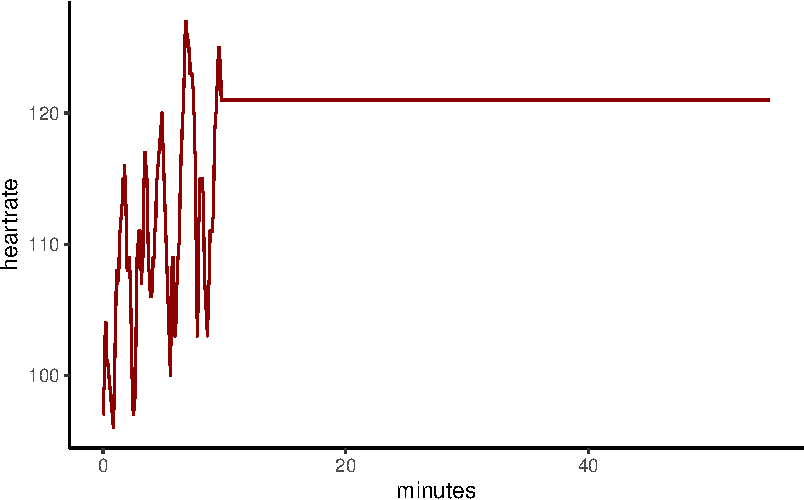
\includegraphics[keepaspectratio]{arrhythmia_files/figure-pdf/sticky_1-1.pdf}}

}

\caption{Extreme example of a sticky heart rate}

\end{figure}%

Clearly, this is not a true picture of the athlete's heart rate!

It can be more subtle. Take this example:

\begin{figure}[H]

{\centering \pandocbounded{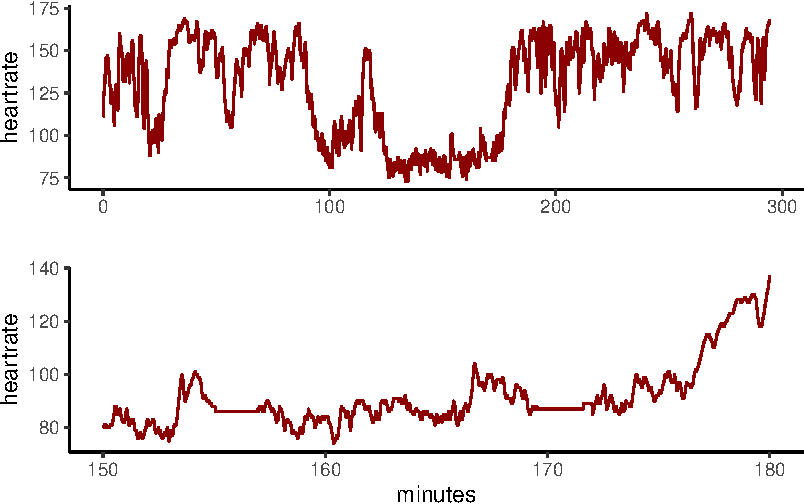
\includegraphics[keepaspectratio]{arrhythmia_files/figure-pdf/sticky_2-1.pdf}}

}

\caption{Subtler case of stickiness}

\end{figure}%

At a first glance, the top chart looks normal. However, if we zoom in,
as we do on the lower chart, we can see a couple of sections where the
reported heart rate is flatlining at a constant level. In fact, it twice
reports a constant level for over two minutes. Again, such flatlining
occurences are physiologically highly implausible yet frequently seen in
the data, even though on longer activities, such as a three hour bike
ride, a couple of minutes of flatlining might not be visually evident on
a chart on a website.

\subsection{Analysis of device by
sport}\label{analysis-of-device-by-sport}

We saw above that we took a sample of over 10,000 activities and
analysed the usage by sport, device and device family. In this sample,
94 different devices were found.

For our purposes, the single most significant difference amongst those
devices that measure heart rate lies between those that measure the
heart rate using electrical sensors near to the heart and those that
measure the pulse optically, typically at the wrist. Studies appear to
show that the former are generally more reliable {[}REF{]}. A related
factor is the frequency with which the heart rate is sampled by the
device. This is a function not only of the device itself but often also
of how it is configured by the user. For example, a bike computer that
is being used to capture readings from a power meter as well as a heart
rate monitor will usually sample data second by second. On the other
hand, running watches will often adjust the sampling frequency
dynamically in order to preserve battery life. We also need to remember
that because of the interoperability between devices and the fact that
we only have one device name (at most) per activity, we only know (at
best) the device used to \emph{record} the heart rate, and we can't
necessarily always strictly deduce from that how the heart rate was
\emph{measured}.

We studied the differences between devices by taking the mean time
between readings for each activity and then finding the median of these
times by device. This gives us the following:

\begin{verbatim}
`summarise()` has grouped output by 'device_family'. You can override using the
`.groups` argument.
\end{verbatim}

\begin{longtable}[]{@{}lrrr@{}}
\caption{Average heart rate sampling frequency in
seconds}\tabularnewline
\toprule\noalign{}
device\_family & Ride & Run & VirtualRide \\
\midrule\noalign{}
\endfirsthead
\toprule\noalign{}
device\_family & Ride & Run & VirtualRide \\
\midrule\noalign{}
\endhead
\bottomrule\noalign{}
\endlastfoot
bike\_computer & 2.0 & 5.0 & 1.1 \\
phone & 1.1 & 1.8 & NA \\
platform & 1.0 & NA & 1.0 \\
trainer & 1.0 & NA & 1.1 \\
watch & 3.2 & 3.6 & 1.0 \\
\end{longtable}

As expected, bike computers used by cyclists have a much lower median
time between readings than watches used by runners. Virtual rides and
rides using a platform or a trainer are very frequently also measuring
power and plugged into a mains supply and it is therefore no surprise to
see that they do second by second sampling.

Runs using a bike computer are rare - there were only 6 in this sample.

Infrequent sampling may be a factor behind a phenomenon often reported
by users of sports watches: the heart rate readings they show tend to
lag the actual heart rate. There are countless instances of this being
reported anecodotally, sometimes by athletes wearing a sports watch and
using a bike computer at the same time specifically to confirm the
phenomenon, but as far as we are aware this has not been studied
systematically.

Insofar as sports watches are laggier than straps, this is most likely
to be observed at low heart rates and at the start of activities when
the heart rate is increasing from a relatively rested state. At the high
end, the heart is unlikely to be able to increase dramatically and in
any case the sampling algorithm is likely to have responed to the
elevated heart rate and to set sampling to a greater frequency. Even so,
it is to eliminate gappiness due to lagged readings that we correlate
arrhythmia with the proportion of \emph{irregular} activities rather
than the proportion of all gappy readings, also including \emph{unclear}
activities.

Our beliefs about the differences between the operation of sports
watches and chest straps lead us to two expectations:

\begin{enumerate}
\def\labelenumi{\arabic{enumi}.}
\tightlist
\item
  Since we believe that watches are laggier than chest straps, we expect
  that the unclear ratio for watches will be higher than for straps;\\
\item
  Since we postulate that irregularity - gappiness only at the high end
  of the range - is in part due to electrical cardiac phenomema, we
  expect that the irregular ratio for straps will be higher than for
  watches.
\end{enumerate}

Both of these expectations are borne out in our sample:

\begin{longtable}[]{@{}lrrr@{}}
\caption{Regularity percentages by device family}\tabularnewline
\toprule\noalign{}
device\_family & irreg\_ratio & strap\_ratio & unclear\_ratio \\
\midrule\noalign{}
\endfirsthead
\toprule\noalign{}
device\_family & irreg\_ratio & strap\_ratio & unclear\_ratio \\
\midrule\noalign{}
\endhead
\bottomrule\noalign{}
\endlastfoot
bike\_computer & 2.7 & 5.1 & 8.2 \\
phone & 0.0 & 11.7 & 3.0 \\
platform & 0.4 & 5.7 & 1.2 \\
trainer & 0.8 & 9.1 & 0.8 \\
watch & 1.9 & 2.1 & 14.8 \\
\end{longtable}

While we would have liked to have been able to select only activities
for which we know that heart rate readings were taken from a chest
strap, we were unable to do so for the reasons explained above and we
believe that selecting only cycling activities in fact achieves this to
an acceptable extent.

\subsection{Residuals}\label{residuals}

In addition to the results shown above, we can analyse leverage and
residuals to evaluate the logistic regression model.

The expected leverage is 0.009434 and should lie between 0 and 1. The
actual values lie between 0.005015 and 0.0779486.

We would expect to see \textasciitilde5\% of the residuals (numerically
= 10.6) have absolute size greater than 1.96; in fact, we see 1.
Likewise, we would expect to see \textasciitilde1\% of the residuals
(numerically = 2.12) have absolute size greater than 2.58; in fact, we
see 0.

\subsection{Data sufficiency}\label{data-sufficiency}

Even after we whittled down our initial population of hundreds of
thousands of activities to those with heart rate data from rides
conducted by survey respondents, we are still left with 207855
activities. These are satisfactorily spread amongst arrhythmics and
non-arrhythmics: the distribution of numbers of filtered activities for
the former is:

\begin{longtable}[]{@{}
  >{\centering\arraybackslash}p{(\linewidth - 10\tabcolsep) * \real{0.0972}}
  >{\centering\arraybackslash}p{(\linewidth - 10\tabcolsep) * \real{0.1389}}
  >{\centering\arraybackslash}p{(\linewidth - 10\tabcolsep) * \real{0.1250}}
  >{\centering\arraybackslash}p{(\linewidth - 10\tabcolsep) * \real{0.1111}}
  >{\centering\arraybackslash}p{(\linewidth - 10\tabcolsep) * \real{0.1389}}
  >{\centering\arraybackslash}p{(\linewidth - 10\tabcolsep) * \real{0.0972}}@{}}
\toprule\noalign{}
\begin{minipage}[b]{\linewidth}\centering
Min.
\end{minipage} & \begin{minipage}[b]{\linewidth}\centering
1st Qu.
\end{minipage} & \begin{minipage}[b]{\linewidth}\centering
Median
\end{minipage} & \begin{minipage}[b]{\linewidth}\centering
Mean
\end{minipage} & \begin{minipage}[b]{\linewidth}\centering
3rd Qu.
\end{minipage} & \begin{minipage}[b]{\linewidth}\centering
Max.
\end{minipage} \\
\midrule\noalign{}
\endhead
\bottomrule\noalign{}
\endlastfoot
43 & 316.2 & 789.5 & 823.8 & 1282 & 2765 \\
\end{longtable}

and for the latter:

\begin{longtable}[]{@{}
  >{\centering\arraybackslash}p{(\linewidth - 10\tabcolsep) * \real{0.0972}}
  >{\centering\arraybackslash}p{(\linewidth - 10\tabcolsep) * \real{0.1389}}
  >{\centering\arraybackslash}p{(\linewidth - 10\tabcolsep) * \real{0.1250}}
  >{\centering\arraybackslash}p{(\linewidth - 10\tabcolsep) * \real{0.0972}}
  >{\centering\arraybackslash}p{(\linewidth - 10\tabcolsep) * \real{0.1389}}
  >{\centering\arraybackslash}p{(\linewidth - 10\tabcolsep) * \real{0.0972}}@{}}
\toprule\noalign{}
\begin{minipage}[b]{\linewidth}\centering
Min.
\end{minipage} & \begin{minipage}[b]{\linewidth}\centering
1st Qu.
\end{minipage} & \begin{minipage}[b]{\linewidth}\centering
Median
\end{minipage} & \begin{minipage}[b]{\linewidth}\centering
Mean
\end{minipage} & \begin{minipage}[b]{\linewidth}\centering
3rd Qu.
\end{minipage} & \begin{minipage}[b]{\linewidth}\centering
Max.
\end{minipage} \\
\midrule\noalign{}
\endhead
\bottomrule\noalign{}
\endlastfoot
6 & 463.8 & 926.5 & 1042 & 1491 & 4189 \\
\end{longtable}

\subsection{Other survey questions}\label{other-survey-questions}

As stated above, the heart health survey captures a number of data
points from respondents. Of these, the only question whose response we
consider in this analysis is \emph{Do you have, or have you had, a heart
rhythym problem?} The relationship between answers to all of the
questions in the survey can be illustrated with an UpSet plot:

\begin{verbatim}
Warning: Removed 1 row containing missing values or values outside the scale range
(`geom_bar()`).
\end{verbatim}

\pandocbounded{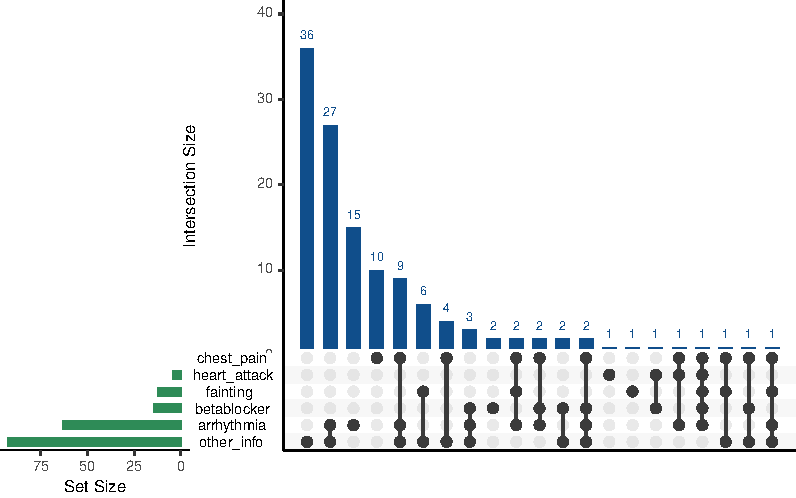
\includegraphics[keepaspectratio]{arrhythmia_files/figure-pdf/upset plot-1.pdf}}

The green bars indicate how many affirmative responses were given to
each question. For example, the bottom two bars tell us that 63
respondents reported arrhythmia and 92 supplied other information (in
free-form text). The heights of the blue columns, also given
numerically, encode the intersection size of affirmative responses as
indicated by the black dots. For example, the first column shows that 24
respondents gave extra information while reporting none of the five
symptoms. Also, if we sum across the columns for which ``other info'' is
given and arrhythmia is also reported we find that there are 42 such
responses.

In future, especially if we have a much larger data set, it may be
fruitful to examine the other symptoms and the free format ``other
information'' for potential explanatory significance.

\subsection{Out of sample test}\label{out-of-sample-test}

Since the original draft of this paper was written the number of survey
responses has increased and it is now more feasible to hold back a
testing set from the sample of surveys. Apportioning 75\% of our surveys
for training and the rest for testing generates the following confusion
matrix on the test set:

\newpage

\begin{longtable}[]{@{}lrr@{}}
\caption{Confusion matrix for an out of sample test set}\tabularnewline
\toprule\noalign{}
Arrhythmia & Predict No & Predict Yes \\
\midrule\noalign{}
\endfirsthead
\toprule\noalign{}
Arrhythmia & Predict No & Predict Yes \\
\midrule\noalign{}
\endhead
\bottomrule\noalign{}
\endlastfoot
No & 37 & 1 \\
Yes & 13 & 2 \\
\end{longtable}

Sensitivity: \textbf{13.3\%}\\
Specificity: \textbf{97.4\%}\\
Positive Predictive Value: \textbf{66.7\%}\\
Negative Predictive Value: \textbf{74\%}

\section{ACKNOWLEDGEMENTS}\label{acknowledgements}

The authors would like to thank Stephen Mildenhall of St John's
University, New York and Mike Bradley of Credit Suisse for helpful
review input.

\section*{REFERENCES}\label{references}
\addcontentsline{toc}{section}{REFERENCES}

\phantomsection\label{refs}
\begin{CSLReferences}{1}{0}
\bibitem[\citeproctext]{ref-Amara2015}
Amara, Mohamed El Oualid. 2015. {``{EARLY DETECTION AND TREATMENT OF
SUPRAVENTRICULAR ARRHYTHMIA WITH REMOTE MONITORING CAN PREVENT ITS
PROGRESSION IN PACEMAKER PATIENTS: THE RANDOMIZED, MULTICENTER SETAM
TRIAL}.''} \emph{Journal of the American College of Cardiology} 65
(10\_Supplement): A388--88.
\url{https://doi.org/10.1016/S0735-1097(15)60388-6}.

\bibitem[\citeproctext]{ref-Baldesberger2008}
Baldesberger, Sylvette. 2008. {``{Sinus node disease and arrhythmias in
the long-term follow-up of former professional cyclists}.''}
\emph{European Heart Journal} 29: 71--78.
\url{https://doi.org/10.1093/eurheartj/ehm555}.

\bibitem[\citeproctext]{ref-Calvo2016}
Calvo, Naiara. 2016. {``{Emerging risk factors and the dose-response
relationship between physical activity and lone atrial fibrillation: a
prospective case-control study}.''} \emph{Oxford University Press on
Behalf of the European Society of Cardiology}.
\url{https://doi.org/10.1093/europace/euv216}.

\bibitem[\citeproctext]{ref-Centurion2019}
Centurión, Osmar Antonio. 2019. {``{The Association Between Atrial
Fibrillation and Endurance Physical Activity: How Much is too Much?}''}
\emph{Journal of Atrial Fibrillation}.
\url{https://doi.org/10.4022/jafib.2167}.

\bibitem[\citeproctext]{ref-Case2017}
Christoper Case, Lennard Zinn, Dr John Mandrola. 2017. \emph{The Haywire
Heart}. 1st ed. Boca Raton, Florida: VeloPress.
\url{https://www.velopress.com/books/the-haywire-heart/}.

\bibitem[\citeproctext]{ref-Tanaka2001}
Hirofumi Tanaka, Kevin D. Monahan, PHD. 2001. {``{Age-Predicted Maximal
Heart Rate Revisited}.''} \emph{Journal of the American College of
Cardiology} 37: 153--56.

\bibitem[\citeproctext]{ref-Kirchhof2009}
Kirchhof, Paulus. 2009. {``{Can we improve outcomes in AF patients by
early therapy?}''} \emph{BMC Medicine}.
\url{https://doi.org/0.1186/1741-7015-7-72}.

\bibitem[\citeproctext]{ref-Perez2019}
Marco V. Perez, Kenneth W. Mahaffey, M. D. 2019. {``{Large-Scale
Assessment of a Smartwatch to Identify Atrial Fibrillation}.''}
\emph{The New England Journal of Medicine}.
\url{https://doi.org/10.1056/NEJMoa1901183}.

\bibitem[\citeproctext]{ref-Tison2018}
Tison, Geoffrey H., José M. Sanchez, Brandon Ballinger, Avesh Singh,
Jeffrey E. Olgin, Mark J. Pletcher, Eric Vittinghoff, et al. 2018.
{``{Passive Detection of Atrial Fibrillation Using a Commercially
Available Smartwatch}.''} \emph{JAMA Cardiology} 3 (5): 409--16.
\url{https://doi.org/10.1001/jamacardio.2018.0136}.

\bibitem[\citeproctext]{ref-Zou2014}
Zou, Ke, Xiaoling; Wang. 2014. {``{Numerical simulations and modeling
for stochastic biological systems with jumps}.''} \emph{Communications
in Nonlinear Science and Numerical Simulation} 19: 1557--68.
\url{https://doi.org/10.1016/j.cnsns.2013.09.010}.

\end{CSLReferences}




\end{document}
